\documentclass[letterpaper,10pt]{article}

\usepackage{titling}
\usepackage{listings}
\usepackage{url}
\usepackage{setspace}
\usepackage{subfig}
\usepackage{sectsty}
\usepackage{pdfpages}
\usepackage{colortbl}
\usepackage{multirow}
\usepackage{relsize}
\usepackage{amsmath}
\usepackage{fancyvrb}
\usepackage{amsmath,amssymb,amsthm,graphicx,xspace}
\usepackage[titlenotnumbered,noend,noline]{algorithm2e}
\usepackage[compact]{titlesec}
\usepackage[default]{droidserif}
\usepackage[T1]{fontenc}
\usepackage{tikz}
\usetikzlibrary{arrows,automata,shapes,trees,matrix,chains,scopes,positioning,calc}
\tikzstyle{block} = [rectangle, draw, fill=blue!20, 
    text width=2.5em, text centered, rounded corners, minimum height=2em]
\tikzstyle{bw} = [rectangle, draw, fill=blue!20, 
    text width=4em, text centered, rounded corners, minimum height=2em]

\definecolor{namerow}{cmyk}{.40,.40,.40,.40}
\definecolor{namecol}{cmyk}{.40,.40,.40,.40}

\let\LaTeXtitle\title
\renewcommand{\title}[1]{\LaTeXtitle{\textsf{#1}}}


\newcommand{\handout}[5]{
  \noindent
  \begin{center}
  \framebox{
    \vbox{
      \hbox to 5.78in { {\bf ECE155: Engineering Design with Embedded Systems } \hfill #2 }
      \vspace{4mm}
      \hbox to 5.78in { {\Large \hfill #4  \hfill} }
      \vspace{2mm}
      \hbox to 5.78in { {\em #3 \hfill} }
    }
  }
  \end{center}
  \vspace*{4mm}
}

\newcommand{\lecture}[3]{\handout{#1}{#2}{#3}{Lecture #1}}
\newcommand{\tuple}[1]{\ensuremath{\left\langle #1 \right\rangle}\xspace}

\addtolength{\oddsidemargin}{-1.000in}
\addtolength{\evensidemargin}{-0.500in}
\addtolength{\textwidth}{2.0in}
\addtolength{\topmargin}{-1.000in}
\addtolength{\textheight}{1.75in}
\addtolength{\parskip}{\baselineskip}
\setlength{\parindent}{0in}
\renewcommand{\baselinestretch}{1.5}
\newcommand{\term}{Spring 2014}

\singlespace


\begin{document}

\lecture{ 10 --- Engineering Design \& Analysis}{\term}{Patrick Lam}

\section*{Engineering Design and Analysis}

Here's the Canadian Engineering Accreditation Board definition of
engineering design:
\vspace{-1em}
\begin{quote}
Engineering design integrates mathematics, basic sciences, engineering sciences, and complementary studies in developing elements, systems, and processes to meet specific needs.  It is a creative, iterative, and often open-ended process subject to constraints which may be governed by standards or legislation to varying degrees depending upon the discipline.  These constraints may relate to economic, health, safety, environmental, social, or other pertinent factors.
\end{quote}

In other words, you have a technical problem and you'd like to solve
it.  Use engineering design. It's an open-ended process which applies
technical knowledge in a creative way for some useful purpose.

\paragraph{Creativity.} 
\begin{quote}
\textit{A good scientist is a person with original ideas.  A good engineer is a person who makes a design that works with as few original ideas as possible.}
\end{quote}
\hfill Freeman Dyson, physicist with mastery of mechanical engineering

\begin{quote}
\textit{I believe that engineering is a highly creative profession. Research tells 
us that creativity does not spring from nothing; it is grounded in our 
life experiences, and hence limited by those experiences. Lacking 
diversity on an engineering team, we limit the set of solutions that 
will be considered and we may not find the best, the \emph{elegant}
solution.}
\end{quote}
\hfill William W. Wulf, former president of National Academy of Engineering

In creativity, we explore a search space for interesting points, perhaps
solutions to a problem.
\begin{itemize}
\item Creativity is required for innovation.
\item Creativity introduces the possibility of failure.
\item A great engineer leverages existing design knowledge as
much as possible and uses creativity only when necessary to solve a problem.
\end{itemize}

\paragraph{Progress.}
\begin{quote} 
\textit{\ldots (that) any general system of conveying passengers would \ldots go at a velocity exceeding ten miles an hour; or thereabouts, is extremely improbable.}
\end{quote}
\hfill Thomas Treadgold, railway engineer, 1835

Progress has been inevitable in the past few hundred years. Engineering
implements technological progress, enabling people to do the improbable.

\paragraph{Engineering Design.}

\begin{quote}
\textit{All parts should go together without forcing.  You must remember that the parts you are reassembling were disassembled by you.  Therefore, if you can't get them together again, there must be a reason.  By all means, do not use a hammer.}
\end{quote}
\hfill IBM Maintenance Manual, 1925

One way of getting a design is by using a (metaphorical) hammer. This is
not going to be a win. Good engineering design is hard.

\paragraph{Overview of the Engineering Design Process.} (i.e. why
people with engineer envy love the waterfall model):

\begin{center}
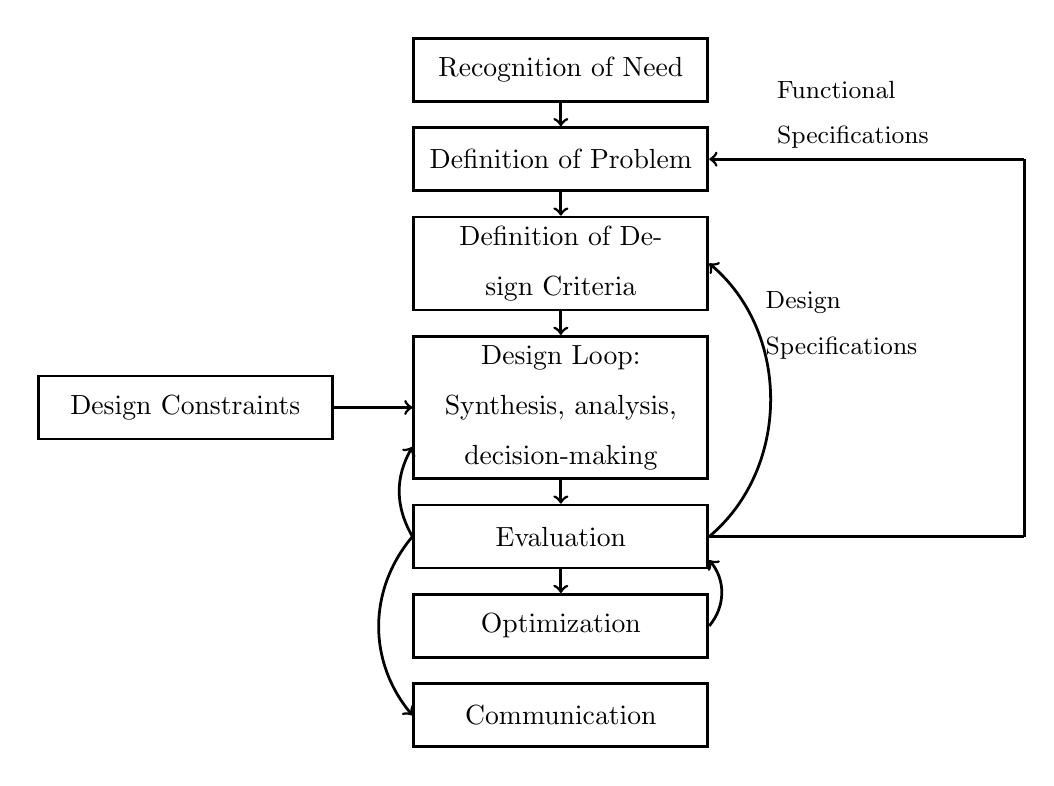
\begin{tikzpicture}
 \matrix (m) [matrix of nodes, column sep=1cm, row sep=0.3cm,
              nodes={draw, line width=1pt, anchor=center,
                     text centered, minimum width=1.5cm, minimum height=8mm},
              txt/.style={text width=3.5cm,anchor=center}
             ]
 { 
  & |[txt]| {Recognition of Need}  \\
  & |[txt]| {Definition of Problem}  \\
  & |[txt]| {Definition of Design Criteria}  \\
 |[txt]| {Design Constraints} & |[txt]| {Design Loop: \\Synthesis, analysis, decision-making}  \\
  & |[txt]| {Evaluation}  \\
  & |[txt]| {Optimization}  \\
  & |[txt]| {Communication}  \\
 };

 { [start chain, ->, every on chain/.style={join}, 
    every join/.style={line width=1pt}]
   \chainin (m-1-2);
   \chainin (m-2-2);
   \chainin (m-3-2);
   \chainin (m-4-2);
   { [start branch=constraints, <-]
     \chainin (m-4-1);
   }
   \chainin (m-5-2);
   \chainin (m-6-2);
 };
 \path[line width=1pt] (m-6-2.east) edge[->, bend right=40] ($ (m-5-2.east) + (0, -0.3) $);
 \path[line width=1pt] (m-5-2.west) edge[->, bend right=40] (m-7-2.west);
 \path[line width=1pt] (m-5-2.east) edge[->, bend right=50] node[near end,right] (ds) {\small \begin{minipage}{6em} Design \\ Specifications\end{minipage}}  (m-3-2.east);
 \path[line width=1pt] (m-5-2.west) edge [->, bend left] ($ (m-4-2.west) + (0, -0.5) $);
% \path[line width=1pt] (m-6-2.east) edge[->, bend right=80] node[near end,right] (ds) {\small \begin{minipage}{6em} Functional \\ Specifications\end{minipage}}  (m-2-2.east);
 \path[line width=1pt] (m-5-2.east) edge ($(m-5-2.east) + (4,0)$)
               ($(m-5-2.east) +(4,0)$) edge ($(m-2-2.east) +(4,0)$)
               ($(m-2-2.east) +(4,0)$) edge[->] node[above] (fs) {\small \begin{minipage}{7em} Functional \\ Specifications \end{minipage} }
                  (m-2-2.east);

\end{tikzpicture}
\end{center}

\paragraph{Note.} This is a model for classical engineering
disciplines, which ends with the transfer of blueprints to
manufacturing/construction firms. Software is different.

\paragraph{Customer Requirements.} In this phase, you're trying to figure
out the properties that the customer is looking for in your solution.
Especially when it comes to software, customers might not know what
they want.  They can give you platitudes, e.g. convenient,
easy-to-use, lightweight, simple. By digging deeper, you can find a design
problem among what they're saying.

Avoid getting pigeonholed by ``helpful'' customers giving you advice on how to solve the problem. See: https://www.youtube.com/watch?v=BKorP55Aqvg

\paragraph{Design Criteria.} Given a problem, you need to know
\emph{specifically} what constitutes a solution. %Examples:
%maximum power consumption (Watts); maximum noise level (decibels);
%minimum transfer rate (bits per second); conforms to standards.
The solution should, to the extent possible, meet the design criteria.
A project that fails to meet one criterion isn't necessarily a failure.

{\sf What are some examples?}


\paragraph{Design Constraints.} Constraints are what make things interesting
(as long as they're satisfiable). The idea is to find a constraint-satisfying
solution.

Design constraints may apply to the design process (that is, the
designer or the final design) or the manufacturing process; they may
be imposed by management, the environment, or physical laws involved
in the design.

{\sf What are some examples of design constraints?}\\[4em]
% project development cost
% physical space constraints
% deadlines for successful complation

We usually consider design constraints non-negotiable; solutions must
satisfy all design constraints.

\paragraph{Heuristics, Guidelines, Standards and Specifications.} 
Here are four related terms.

A \emph{design heuristic} is a general (and not necessarily
actionable) rule-of-thumb based on experience.  Heuristics lead to
quick design solutions that often work well but may fail in some
situations. No substitute for understanding.

A \emph{design guideline} is a general rule based on experience and
specific knowledge of the design problem that may be applied to a design
solution. When we talk about guidelines, we mean something more specific
than heuristics.

A \emph{standard} provides more direction about the acceptable
solution space by stating technical requirements that must be satisfied
by candidate designs. Standards do not provide a complete solution, but 
do dictate a set of requirements that must be satisfied by a solution.

Our definition of \emph{specification} refers to a description of a solution
which provides all of the details. Using a specification, an engineer
should be able to reproduce a design exactly.

{\sf What are examples of all of these terms?} \\[6em]

\paragraph{Synthesis, Analysis and Decision-Making.} Now you know about
your constraints and requirements. Time to come up with a solution.
You will use the \emph{design loop}.

\begin{itemize}
\item Synthesis: gather information, combine (synthesize) it, and come up
with ideas or methods to solve a problem.
\item Analysis: estimate the expected result from each idea or method.
\item Decision-making: compare the expected results and their uncertainties; pick the best alternative.
\end{itemize}

You'll find that you often have to iterate the design loop. Even after you
get a ``best'' alternative, you might have found that your criteria were 
wrong, or that you didn't satisfy all of the design constraints or meet
the desired design criteria.

When iterating, you bring the less-favoured alternatives back on the table,
and reconsider and revise all of the alternatives. You'll get a better set
of alternatives out of the process.

Once you have a sufficiently-good best design, you can finish the
design loop. This design should satisfy all constraints and achieve the
desired criteria. Choose the winning design, optimize, and implement it.

\paragraph{Innovation versus evolution.} Solutions tend to have some
innovation and some evolution. It's a continuum.
\begin{itemize}
\item Evolutionary design solutions \emph{build on top of} existing solutions,
improving them in some way.
\item Innovative design solutions invent \emph{something new}, a completely
original idea or a novel way of solving the design problem.
\end{itemize}

Modern engineering design solutions combine innovation and evolution. 
(You don't want to innovate on all fronts simultaneously). 
Consider, for instance, the Brooklyn Bagel Slicer:

~~~~\url{http://online.wsj.com/article/SB125952152870368561.html}

~~~~\url{http://www.amazon.com/Brooklyn-Bagel-Slicer-Knife-Stainless/dp/B001PN0GBE}

It is a knife embedded in plastic to enable you to safely cut bagels,
while avoiding Bagel-Related Injuries. 

{\sf What is innovative about this design? What is evolutionary?}
\\[4em]

\paragraph{Creativity.} One of the popular misconceptions about
engineering is that it's not creative. Good engineering uses creativity
when necessary.

The best engineers know when to be innovative and when to simply build 
upon the designs of others. Creativity should be avoided when it doesn't
pay off, and non-standard (creative) solutions need to be carefully
analyzed to ensure that they meet all requirements and constraints,
potentially add to the time required to complete a design and to the cost
required to prototype a design.

The risks of creativity, then, are that you might not find anything,
and that you might get something unsatisfactory.

Here are five steps in a typical creative process:
\begin{enumerate}
\item Gather information.
\item Make a concentrated mental effort to understand the problem.
\item Take a break (sleep, do something else, take a shower, etc.)
\item Discover the solution to the problem (often subconscious).
\item Write down the solution and refine it.
\end{enumerate}

There is reason to believe that generating lots of alternatives (or,
on a related topic, getting lots of practice developing 
skills \cite{lifeClever, lifeclever2}) is
better than trying to come up with the one ideal solution.

\paragraph{Brainstorming and Brainwriting.} Here are two techniques for
generating ideas; you've probably heard of brainstorming.

The usual part of brainstorming is the synthesis part, where you write
down all ideas. But there's also an analysis part, where you go over the 
ideas.

\begin{itemize}
\item Synthesis: come up with new ideas synthesizing the information;
don't discount any ideas, just write them down.
\item Analysis: look at all of the ideas (to some extent) and analyze them. Determine the most promising solutions.
\end{itemize}
Because unusual ideas show up, and aren't immediately discounted, 
they can help you come up with a variety of creative solutions, some of 
which might turn out to be practical.

Brainwriting is similar to brainstorming, but involves more paper.
\begin{itemize}
\item Write down tentative solutions on \emph{solution sheets}.
\item Each team member picks a solution sheet to refine.
\item Exchange solution sheets until members run out of ideas.
\end{itemize}
Because you're writing things down, you can avoid dropping things on the floor.

\paragraph{Avoiding getting stuck.} Roger von 
Oech \cite{creativeThink} produces a lot of
output about creativity. According to him, here are some mistaken
beliefs that people often have.

\begin{itemize}
\item There is only one right answer.
\item The creative process must be logical.
\item They must ``follow the rules'' even if the rules are unwritten.
\item They must be practical and therefore inhibit their fantasies.
\item They must avoid ambiguity and therefore stifle their imagination.
\item They avoid new ideas for fear of making mistakes.
\item Play is frivolous, and new ideas are hard work.
\item They narrow their focus and miss ideas in nearby areas.
\item They are afraid to look foolish by suggesting an unworkable idea.
\item They are not creative.
\end{itemize}

\section*{Evaluation}
Moving on, let's talk about the evaluation phase of the design
process.  Now you have one or more candidate designs (design
alternatives) and want to see how good it is.

A \emph{design review} is an independent evaluation of a design alternative:
\begin{itemize}
\item act as a ``sanity check'' on the design; and 
\item are often conducted by evaluation teams consisting of clients and/or
managers.
\end{itemize}
If all alternatives are bad (failed design reviews), the client might
terminate the project.

Evaluation teams will consider the following questions:
\begin{itemize}
\item Does the design team have a thorough understanding of the purpose and goals of the design?
\item Have all of the relevant requirements, criteria, and constraints been identified?
\item Is the overall design plausible for meeting the design objectives?
\item Does the overall design appear to meet the criteria specified?
\item Is the (anticipated) performance of the design adequate?
\item Are there any flaws in the analysis of the design?
\end{itemize}

\paragraph{Design Alternatives} Consider presenting more than one alternative
at a design
review. In
the presence of unclear requirements or in a large search space,
having alternatives can help the customer pick the best alternative,
rather than just saying ``I don't like your solution''. Also, trying
to push bad designs forward can help you understand why those designs
are bad.

\section*{Communication} The last phase of the engineering design 
process (and many other creative endeavours) is communication. You
haven't done anything if you don't (successfully) tell anyone about
it. But communication is also important en-route.

\paragraph{Communication between stakeholders} 
The designers/implementers, managers, and clients need to communicate.
Without communication, people tend to assume that things are going well,
which can lead to unmet expectations and unpleasant surprises.

\paragraph{Intra-team communication.} You also need
communication within the design team. For a small team, communication
helps with continuity and allows you continue the project even if an
engineer leaves the company. (This is a key reason that extreme
programming, which we'll see later, plays up communication so
much). For a large team, communication is mandatory for making sure
that all of the parts integrate and for tracking the schedule.

\section*{Design Team Organization}
Here are some considerations to keep in mind when organizing and managing
design teams.

\begin{itemize}
\item Keep team sizes small; Amazon uses the ``two-pizza'' team concept,
splitting large projects into smaller ones. Their team size is at most
8--10. Larger teams have too much coordination overhead.
\item Consider how you want to divide responsibility. Extreme
  programming advocates collective code ownership; traditional models
  allocate responsibility for specific parts of the project to
  specific people.
\item Ensure that each team member's contribution is important and
  that each team member understands how their part of the design
  contributes to the overall goal.
\item Set up open communication, so that all members understand
  relevant schedules, deadlines, and intermediate objectives, and
  proactively track team members' progress. (Don't pester!)
\item Encourage creativity when necessary, but make sure team members
  aren't going overboard.
\end{itemize}

\paragraph{Potential dysfunctions.} Per Steve McConnell, \emph{Rapid Development}, 
pp. 156--168, Microsoft Press, 1996.
\begin{itemize}
\item Lack of common vision
\item Lack of identity
\item Lack of recognition
\item Productivity roadblocks
\item Ineffective communication
\item Lack of trust
\item Problem personnel
\end{itemize}

\paragraph{Typical Set of Design Groups.} Here are some design groups
that a large organization might use.

\begin{itemize}
\item Development Group: tests the feasibility of new technologies and ideas.
\item Design Group: refines a design to ensure manufacturability, reliability, safety, and efficient operation.
\item Manufacturing Group: refines a design based on the results of the manufacturing process and the performance of test batches.
\item Quality Control Group: monitors the quality of products in wide use.
\item Customer Service Group: tracks the performance of products and ongoing maintenance performed for customers.
\end{itemize}

In reality, design groups work concurrently and must sometimes
synchronize their work. 

Development, design, manufacturing, quality control, and customer
service tasks often require many groups to work together. Since these
groups may have different goals and deadlines, consensus and
cooperation may be difficult to achieve. (In fact, organizational
inertia generally makes inter-group cooperation difficult, even
without different goals and deadlines.)

Project management attempts to ensure that all groups work together as
a cohesive unit. Time management is particularly important for any
project with many cooperating teams; this includes scheduling meetings
and deadlines.



\bibliographystyle{alpha}
\bibliography{155}


\end{document}
